\section{Análisis Empírico}

\subsection{\textit{\textbf{Entradas de prueba}}}

En este escenario, se emplearon 30 entradas para el algoritmo basado en el enfoque de programación dinámica. Esta elección se realizó debido a que dicho enfoque tiene una complejidad temporal asintótica de \(O(n^{2})\). Por otro lado, utilizar las mismas entradas para el enfoque de Divide and Conquer resultaba virtualmente imposible, ya que este algoritmo presenta una complejidad polinomial de base 3 dependiente del tamaño de la entrada. Como consecuencia, su ejecución requeriría tiempos de cómputo extremadamente largos.\\

Por lo tanto, se optó por utilizar dos conjuntos de pruebas diferentes. El primero consistió en una serie de cadenas de prueba que variaban en longitud desde 8 hasta 9000 caracteres. Se realizaron un total de 30 pruebas en este conjunto. Por otro lado, el segundo conjunto constaba de 12 pruebas con cadenas cuya longitud iba desde 2 hasta 13 caracteres.\\

El primer conjunto mencionado puede ser hayado en el siguiente enlace (30 pruebas): \url{https://github.com/OrtegaRehbach/Proyecto02ADA/tree/main/sequence_hard}\\

El segundo conjunto de pruebas mencionado puede ser hayado en el siguiente enlace (12 pruebas): \url{https://github.com/OrtegaRehbach/Proyecto02ADA/tree/main/sequence_easy}

\subsection{\textit{\textbf{Gráficas}}}

\begin{center}
\fbox{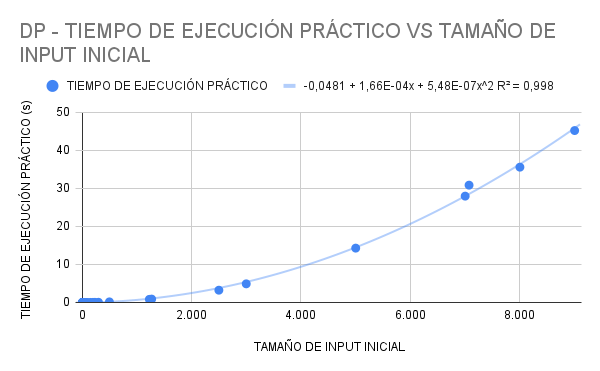
\includegraphics[width=15cm, height=9cm,]{images/DP - TIEMPO DE EJECUCIÓN PRÁCTICO VS TAMAÑO DE INPUT INICIAL .png}}\\
\vspace{0.02in}
\small\textcolor{FSBlue}{Gráfica 1: Programación Dinámica, Tiempo Práctico vs Tamaño de Input}.
\end{center}

\begin{center}
\fbox{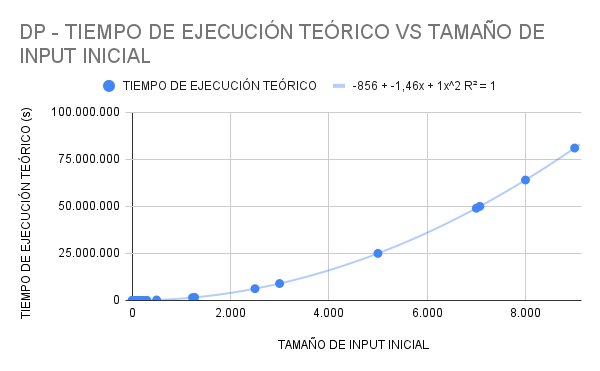
\includegraphics[width=15cm, height=9cm,]{images/DP - TIEMPO DE EJECUCIÓN TEÓRICO VS TAMAÑO DE INPUT INICIAL .png}}\\
\vspace{0.02in}
\small\textcolor{FSBlue}{Gráfica 2: Programación Dinámica, Tiempo Teórico vs Tamaño de Input}.
\end{center}

\begin{center}
\fbox{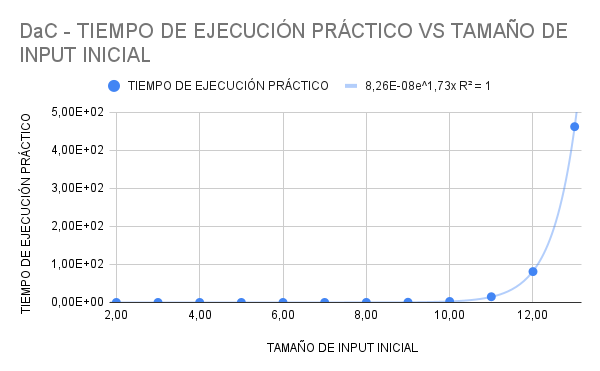
\includegraphics[width=15cm, height=9cm,]{images/DaC - TIEMPO DE EJECUCIÓN PRÁCTICO VS TAMAÑO DE INPUT INICIAL .png}}\\
\vspace{0.02in}
\small\textcolor{FSBlue}{Gráfica 3: Divide and Conquer (12 Pruebas), Tiempo Práctico vs Tamaño de Input}.
\end{center}

\begin{center}
\fbox{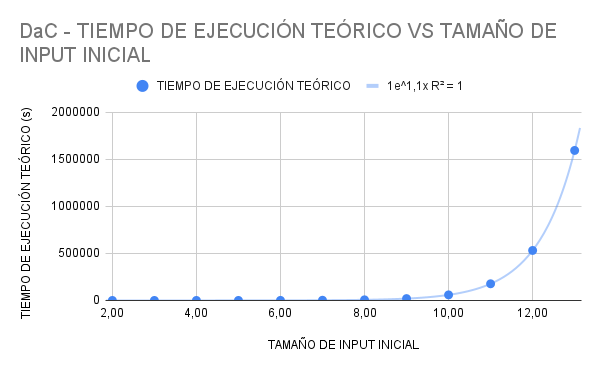
\includegraphics[width=15cm, height=9cm,]{images/DaC - TIEMPO DE EJECUCIÓN TEÓRICO VS TAMAÑO DE INPUT INICIAL .png}}\\
\vspace{0.02in}
\small\textcolor{FSBlue}{Gráfica 4: Divide and Conquer (12 Pruebas), Tiempo Teórico vs Tamaño de Input}.
\end{center}

\begin{center}
\fbox{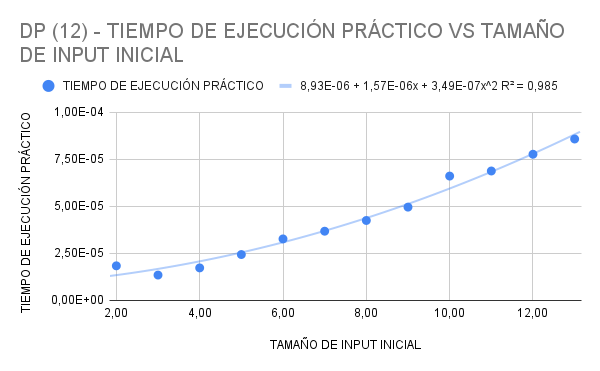
\includegraphics[width=15cm, height=9cm,]{images/DP (12) - TIEMPO DE EJECUCIÓN PRÁCTICO VS TAMAÑO DE INPUT INICIAL .png}}\\
\vspace{0.02in}
\small\textcolor{FSBlue}{Gráfica 5: Programación Dinámica (12 Pruebas), Tiempo Práctico vs Tamaño de Input}.
\end{center}

\begin{center}
\fbox{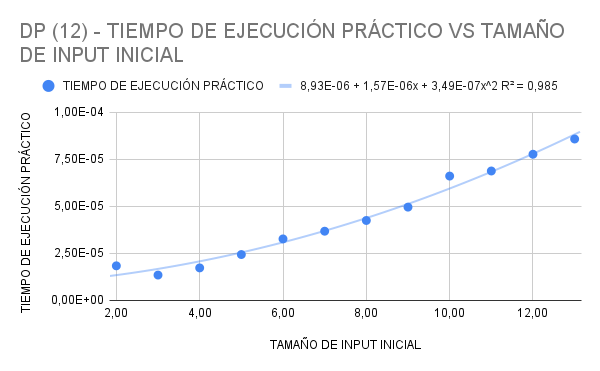
\includegraphics[width=15cm, height=9cm,]{images/DP (12) - TIEMPO DE EJECUCIÓN PRÁCTICO VS TAMAÑO DE INPUT INICIAL .png}}\\
\vspace{0.02in}
\small\textcolor{FSBlue}{Gráfica 6: Programación Dinámica (12 Pruebas), Tiempo Teórico vs Tamaño de Input}.
\end{center}

\subsection{\textit{\textbf{Comentarios}}}

Las Gráficas 1 y 2 representan los resultados obtenidos para el primer conjunto de pruebas al utilizar el algoritmo programación dinámica. Se observa que los resultados prácticos se ajustan con un coeficiente R cercano a 1 en una regresión polinomial de segundo grado. Esto concuerda con la complejidad teórica medida en \(O(m∗n)\), donde en la mayoría de las pruebas las cadenas tenían tamaños similares, por lo que la complejidad se puede aproximar a \(O(n^{2})\). En base a esto, podemos sugerir que los resultados empíricos respaldan y concuerdan con las predicciones teóricas.\\

Las Gráficas 3 y 4 muestran los resultados obtenidos para el segundo conjunto de pruebas al utilizar el algoritmo de enfoque \quotes{Divide and Conquer}. Los resultados del tiempo de ejecución práctico coinciden con las expectativas teóricas de complejidad, lo cual se evidencia al aplicar una regresión exponencial correspondiente a una medida teórica de \(O(3^{n})\). No se observa ninguna discrepancia significativa entre los resultados empíricos y los resultados teóricos. En base a esto, podemos sugerir que los resultados empíricos respaldan y concuerdan con las predicciones teóricas, indicando una coherencia entre ambos. Es importante destacar que debido a la alta complejidad de este algoritmo, no fue posible realizar simulaciones con cadenas más largas, ya que se evidencia que a partir de 12 caracteres, como se observa en la Gráfica 3, el tiempo de ejecución crece rápidamente.\\

Las Gráficas 5 y 6 representan nuevamente los resultados de pruebas al utilizar el algoritmo de enfoque de programación dinámica, pero con el segundo conjunto de pruebas. Al igual que en las gráficas anteriores (Gráficas 1 y 2), se observa que no existe una discrepancia significativa entre las predicciones teóricas y los resultados empíricos.\\